\newcommand{\malwareResultsAucTable}{
    \begin{table}[H]
        \centering
        \begin{tabular}{|p{2,8cm}||p{2,8cm} p{2,8cm} p{2,8cm}|}
            \hline
            Malware Label & ALOHA & Joint Embedding & Proposed Model \\
            \hline
            AUC-ROC & \textBF{0.646$\pm$0.016} & - & 0.631$\pm$0.013 \\
            \hline
        \end{tabular}
        \caption{AUC-ROC (Area Under Curve) of the different models for the \textbf{Malware Label} prediction task. Results were aggregated over \textBF{3} training runs with different weight initializations and minibatch orderings. Best results are shown in \textbf{bold}.} \label{tab:malware_auc}
    \end{table}
}

\newcommand{\malwareResultsAtFprTable}{
    \begin{center}
        \begin{longtable}[c]{|p{3,2cm}||p{1,8cm} p{1,8cm} p{1,8cm} p{1,8cm} p{1,8cm}|}
            \hline
            Malware Label & \multicolumn{5}{c|}{{FPR}} \\
            & $10^{-5}$ & $10^{-4}$ & $10^{-3}$ & $10^{-2}$ & $10^{-1}$ \\
            \hline
            \endfirsthead

            \caption*{\raggedright ...continued from previous page} \\
            \hline
            Malware Label & \multicolumn{5}{c|}{\textbf{FPR}} \\
            & $10^{-5}$ & $10^{-4}$ & $10^{-3}$ & $10^{-2}$ & $10^{-1}$ \\
            \hline
            \endhead

            \caption*{\raggedleft ...continued on next page} \\
            \endfoot

            \caption{Mean and standard deviation results (TPR, Accuracy, Recall, Precision and F1-Score) of the different models for the \textbf{Malware Label} prediction task at different \textbf{FPR}s (\textit{False Positive Rates}). Results were aggregated over \textBF{3} training runs with different weight initializations and minibatch orderings. Best results are shown in \textbf{bold}. Under \textbf{TPR} results are also presented the percentage reduction in mean detection error and in ROC curve standard deviation introduced by the \textit{Proposed Model} with respect to both \textit{ALOHA} model and \textit{Joint Embedding}.} \label{tab:malware_results_at_fpr} \\
            \endlastfoot

            \multicolumn{6}{|c|}{\textbf{TPR}} \\
            \hline
            ALOHA & \textBF{0.014$\pm$0.008} & \textBF{0.014$\pm$0.008} & \textBF{0.014$\pm$0.008} & \textBF{0.039$\pm$0.015} & \textBF{0.212$\pm$0.017} \\
            Joint Embedding & - & - & - & - & - \\
            Proposed Model & 0.001$\pm$0.000 & 0.001$\pm$0.000 & 0.004$\pm$0.002 & 0.031$\pm$0.003 & 0.174$\pm$0.008 \\
            \hline
            Error Reduction wrt \newline ALOHA & -1.3\% & -1.3\% & -1.0\% & -0.8\% & -4.8\% \\
            Error Reduction wrt \newline Joint Embedding & - & - & - & - & - \\
            \hline
            Std Reduction wrt \newline ALOHA & 100.0\% & 100.0\% & 75.0\% & 80.0\% & 52.9\% \\
            Std Reduction wrt \newline Joint Embedding & - & - & - & - & - \\
            \hline
            \multicolumn{6}{|c|}{\textbf{Accuracy}} \\
            \hline
            ALOHA & \textBF{0.716$\pm$0.002} & \textBF{0.716$\pm$0.002} & \textBF{0.716$\pm$0.002} & \textBF{0.717$\pm$0.004} & \textBF{0.703$\pm$0.005} \\
            Joint Embedding & - & - & - & - & - \\
            Proposed Model & 0.713$\pm$0.000 & 0.713$\pm$0.000 & 0.713$\pm$0.001 & 0.714$\pm$0.001 & 0.691$\pm$0.002 \\
            \hline
            \multicolumn{6}{|c|}{\textbf{Recall}} \\
            \hline
            ALOHA & \textBF{0.014$\pm$0.008} & \textBF{0.014$\pm$0.008} & \textBF{0.014$\pm$0.008} & \textBF{0.039$\pm$0.015} & \textBF{0.212$\pm$0.017} \\
            Joint Embedding & - & - & - & - & - \\
            Proposed Model & 0.001$\pm$0.000 & 0.001$\pm$0.000 & 0.004$\pm$0.002 & 0.031$\pm$0.003 & 0.174$\pm$0.008 \\
            \hline
            \multicolumn{6}{|c|}{\textbf{Precision}} \\
            \hline
            ALOHA & \textBF{1.000$\pm$0.000} & \textBF{1.000$\pm$0.000} & \textBF{0.852$\pm$0.073} & \textBF{0.598$\pm$0.097} & \textBF{0.463$\pm$0.020} \\
            Joint Embedding & - & - & - & - & - \\
            Proposed Model & \textBF{1.000$\pm$0.000} & \textBF{1.000$\pm$0.000} & 0.667$\pm$0.136 & 0.558$\pm$0.021 & 0.413$\pm$0.012 \\
            \hline
            \multicolumn{6}{|c|}{\textbf{F1 Score}} \\
            \hline
            ALOHA & \textBF{0.027$\pm$0.016} & \textBF{0.027$\pm$0.016} & \textBF{0.028$\pm$0.015} & \textBF{0.074$\pm$0.026} & \textBF{0.291$\pm$0.020} \\
            Joint Embedding & - & - & - & - & - \\
            Proposed Model & 0.003$\pm$0.000 & 0.003$\pm$0.000 & 0.008$\pm$0.005 & 0.059$\pm$0.006 & 0.245$\pm$0.010 \\
            \hline
        \end{longtable}
    \end{center}
}

\newcommand{\malwareResultsSummaryTable}{
    \begin{table}[H]
        \centering
        \begin{tabular}{|p{3,2cm}||p{1,8cm} p{1,8cm} p{1,8cm} p{1,8cm} p{1,8cm}|}
            \hline
            \multicolumn{6}{|c|}{Malware Label (at FPR $=1\%$)} \\
            \hline
            Model & TPR & Accuracy & Precision & Recall & F1 score \\
            \hline
            ALOHA & \textBF{0.039$\pm$0.015} & \textBF{0.717$\pm$0.004} & \textBF{0.598$\pm$0.097} & \textBF{0.039$\pm$0.015} & \textBF{0.074$\pm$0.026} \\
            Joint Embedding & - & - & - & - & - \\
            Proposed Model & 0.031$\pm$0.003 & 0.714$\pm$0.001 & 0.558$\pm$0.021 & 0.031$\pm$0.003 & 0.059$\pm$0.006 \\
            \hline
        \end{tabular}
        \caption{Summary of the mean and standard deviation results of the different models for the \textbf{Malware Label} prediction task at \textbf{FPR} $=1\%$. Results were aggregated over \textBF{3} training runs with different weight initializations and minibatch orderings. Best results are shown in \textbf{bold}.} \label{tab:malware_result_summary}
    \end{table}
}

\newcommand{\malwareRocAloha}{
    \begin{figure}[H]
        \vspace*{-0.5cm}
        \centering
        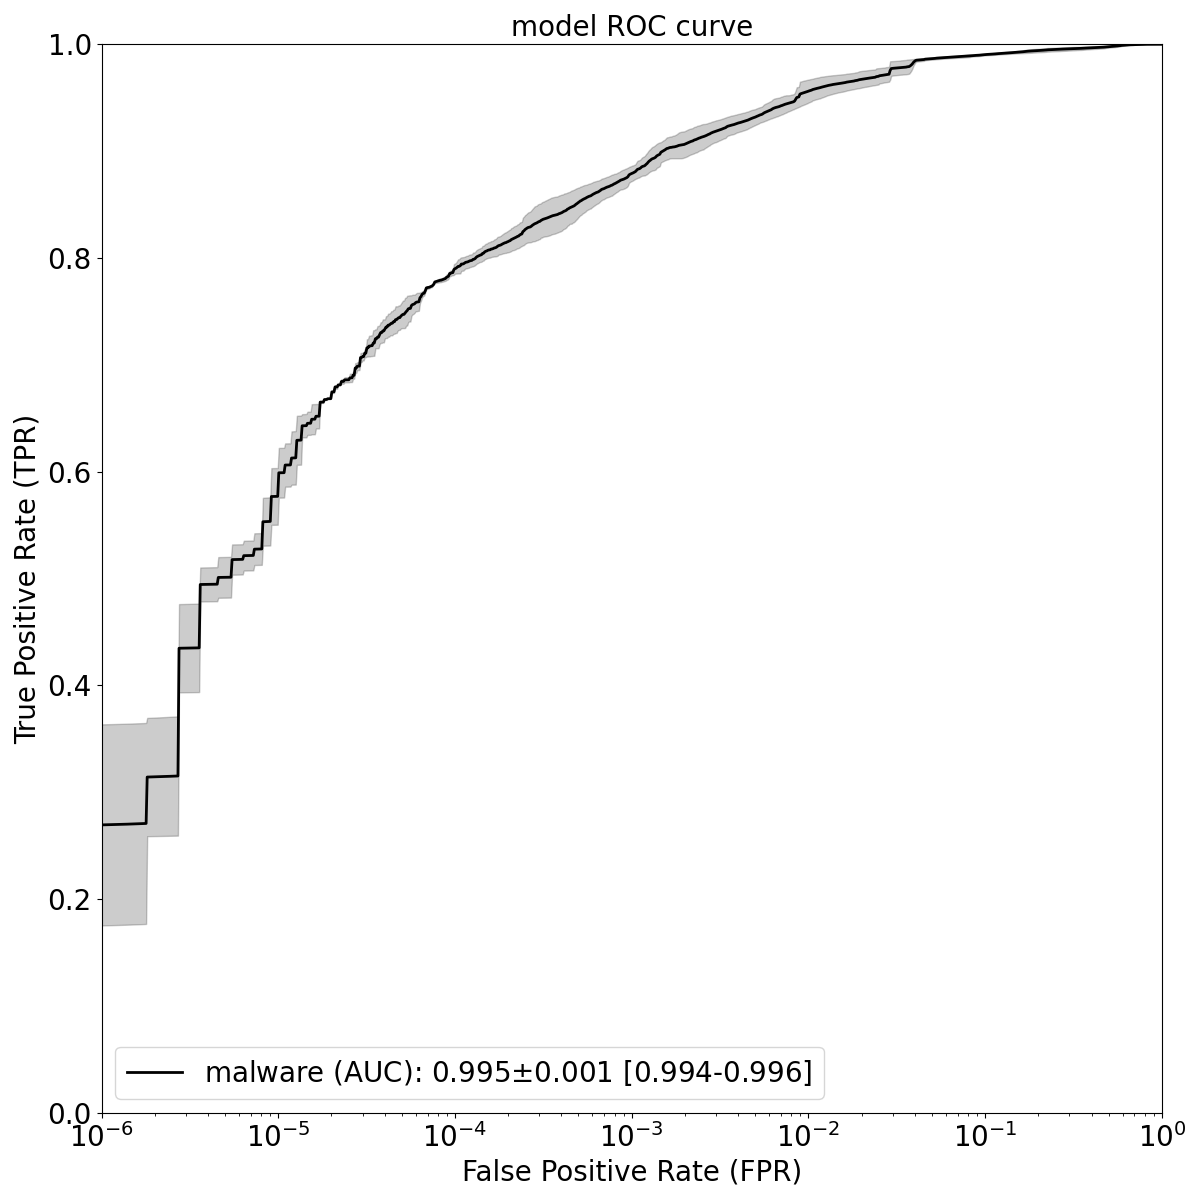
\includegraphics[width=0.6\textwidth]{./results/malware_roc_aloha.png}
        \vspace*{-0.2cm}
        \caption{ROC curve and AUC statistics of \textBF{ALOHA} model for the \textbf{Malware Label}. The line represents the \textit{mean} TPR at a given FPR, while the shaded region represents the \textit{standard deviation}. Statistics were computed over \textBF{3} training runs, each with random parameter initialization.}
        \label{fig:malwareRocAloha}
    \end{figure}
}

\newcommand{\malwareRocJointEmbedding}{
    \begin{figure}[H]
        \vspace*{-0.5cm}
        \centering
        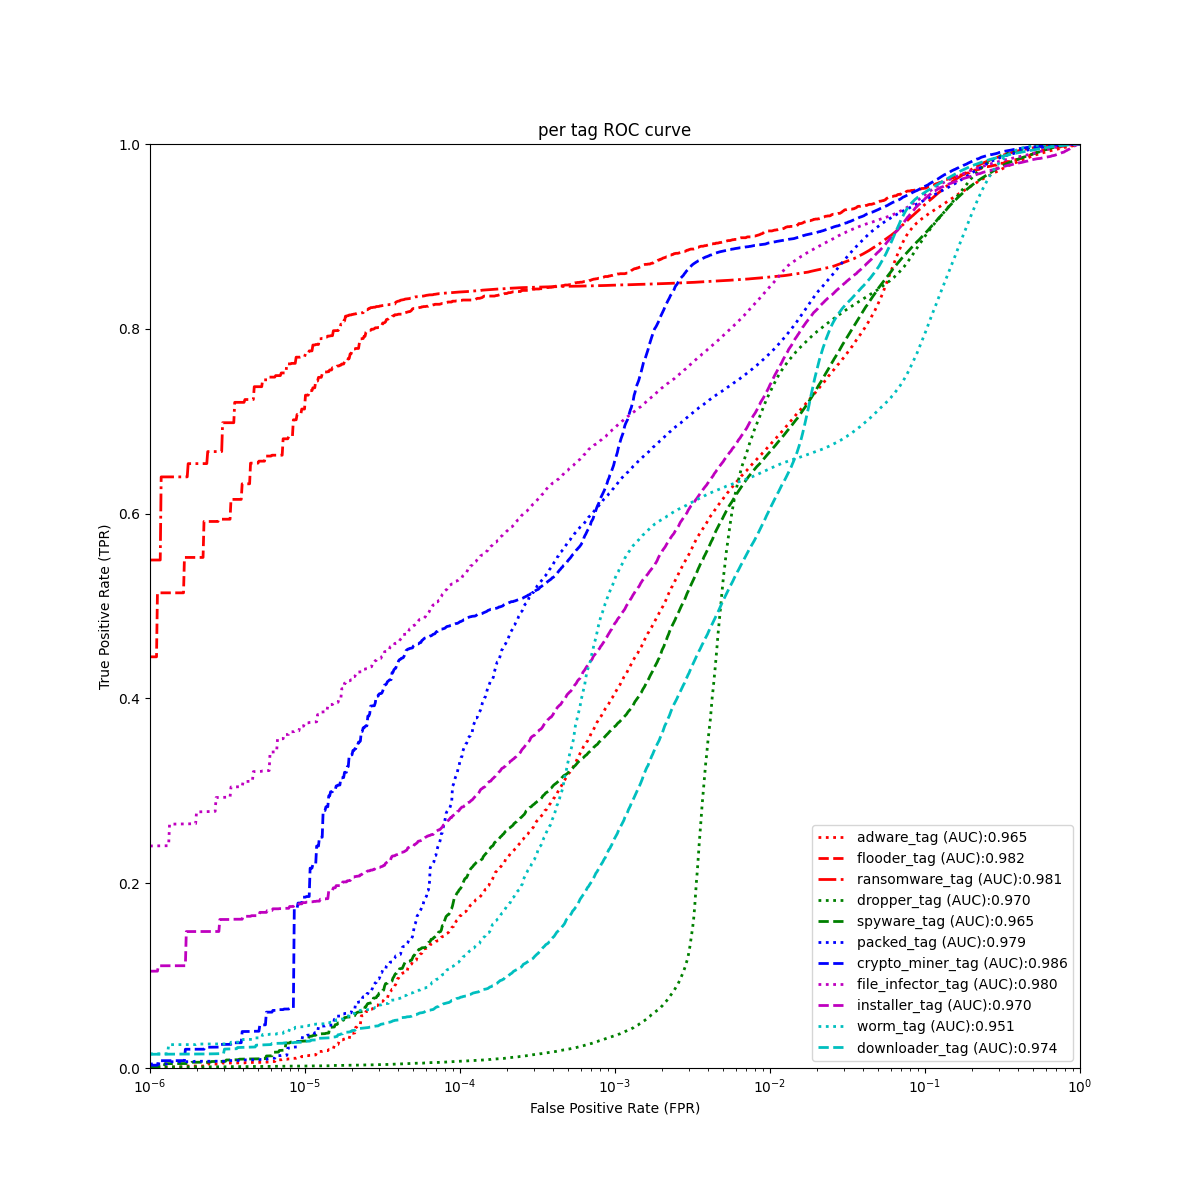
\includegraphics[width=0.6\textwidth]{./results/malware_roc_jointEmbedding.png}
        \vspace*{-0.2cm}
        \caption{ROC curve and AUC statistics of \textBF{Joint Embedding} model for the \textbf{Malware Label}. The line represents the \textit{mean} TPR at a given FPR, while the shaded region represents the \textit{standard deviation}. Statistics were computed over \textBF{3} training runs, each with random parameter initialization.}
        \label{fig:malwareRocJointEmbedding}
    \end{figure}
}

\newcommand{\malwareRocProposedMethod}{
    \begin{figure}[H]
        \vspace*{-0.5cm}
        \centering
        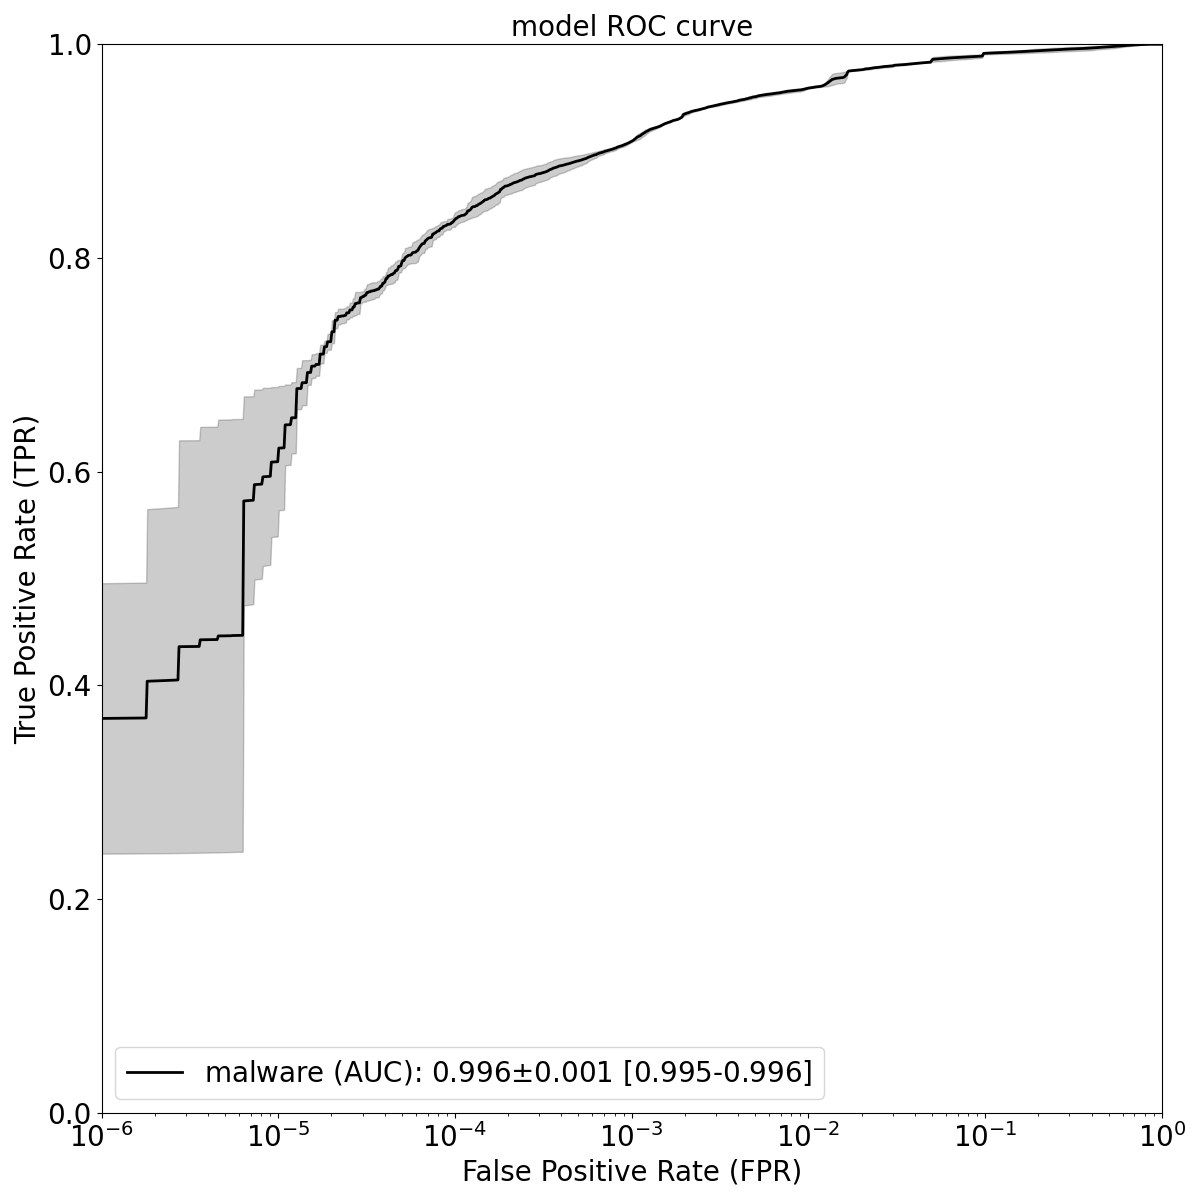
\includegraphics[width=0.6\textwidth]{./results/malware_roc_proposedModel.png}
        \vspace*{-0.2cm}
        \caption{ROC curve and AUC statistics of \textBF{Proposed Model} for the \textbf{Malware Label}. The line represents the \textit{mean} TPR at a given FPR, while the shaded region represents the \textit{standard deviation}. Statistics were computed over \textBF{3} training runs, each with random parameter initialization.}
        \label{fig:malwareRocProposedModel}
    \end{figure}
}
